\section{Auswertung}
\subsection{Analyse der Stabilität}
Durch die Darstellung der Stabilitätsbedingung aus Gleichung \ref{eq:stabil} der jeweiligen Spiegelkonfiguration
lässt sich durch die Messungen aus Tabelle \ref{tab:stabil} die folgenden Aussagen treffen.

Für die beiden Speigelkonfigurationen konkav/konkav (mit $r_1=r_2=1400\,$mm) und plan/konkav ($r_1=\infty {,} r_2=1400\,$mm)
lässt sich das Stablitätsprodukt $g_1g_2$ gegen die Resonatorlänge $L$.
Extrapoliert man die Messwerte mit hilfe der geeigneten Funktion die aus Gleichung \ref{eq:stabil} hervorgeht (Linear- und Quadratfunktion)
so ergibt sich für die konkav/konkav Konfiguration die theoretische maximale Resonatorlänge von $L_{\text{max}}=2,80\,$m (in Abbildung \ref{fig:stabil} in rot dargestellt), 
sowie eine kritische Stabilität bei $L_{\text{kri}}=1,40\,$m. 

\begin{figure}[H]
    \center
    \includegraphics[width=\textwidth]{plots/stabilitätsbedingung.pdf}
    \caption{Das Stabilitätsprodukt $g_1g_2$ der beiden Spiegelkonfigurationen (konkav/konkav in blau und plan/konkav in gelb) mit der jewiligen Extrapolation (gestrichelt blau/gelb).
    Die kritischen Stabilitäten sind durch die rot geschrichelten Linin hervorgehoben.}
    \label{fig:stabil}
\end{figure}
\label{sec:Auswertung}

Die jeweilige gemessene Leistung $P$ bei betrachteter Resonatorlänge $L$ ist der Tabelle \ref{tab:stabil} und 
der Abbildung \ref{fig:leistung} zu entnehmen. Es wird deutlich, dass die Konfiguration der konkav/konkav Spiegeln keine Resonatorlänge $L$ gefunden 
werden kann für diese der Laserbetreib nicht aufrecht gehalten werden kann. Eine Aussage über die plan/konkave Konfiguration 
lässt sich aufgrund der Daten nicht treffen.

\begin{table}
    \center
    \caption{Messwerte der beiden Spiegelkonfigurationen. Gemessen wurde die Leistung $P$ in Abhängigkeit der Resonatorlänge $L$.}
    \begin{tabular}{c c | c c}
        \multicolumn{2}{|c|}{konkav/konkav} &\multicolumn{2}{|c|}{plan/konkav} \\
        \hline
        $L\,/\,$cm & $P\,/\,$mW & $L\,/\,$cm & $P\,/\,$mW\\
        \midrule
        61.5&        2.36&  60& 1.28\\
        65  &        2.57&  65& 1.43\\
        70  &        2.87&  70& 1.54\\
        75  &        2.99&  75& 1.67\\
        80  &        2.91&  80& 1.75\\
        85  &        2.82&  85& 1.84\\
        90  &        2.7&   90& 2.14\\
        95  &        2.28&  95& 2.38\\
        100 &        2.46&  100&2.33\\
        105 &        2.27&  105&2.48\\
        110 &        2.30&  110&2.64\\
        115 &        2.27&  115&2.72\\
        120 &        2.11&  120&2.72\\
        125 &        2&     125&2.57\\
        130 &        2&     130&2.57\\
        140 &        2.16&  &\\
        150 &        1.46&  &\\
        160 &        1.6&  &\\
        170 &        1.92&  &\\
        175 &        2.1&  &\\
        180 &        2.71&  &\\
        190 &        3.35&  &\\
        \bottomrule
    \end{tabular}
    \label{tab:stabil}
\end{table}

\begin{figure}[H]
    \center
    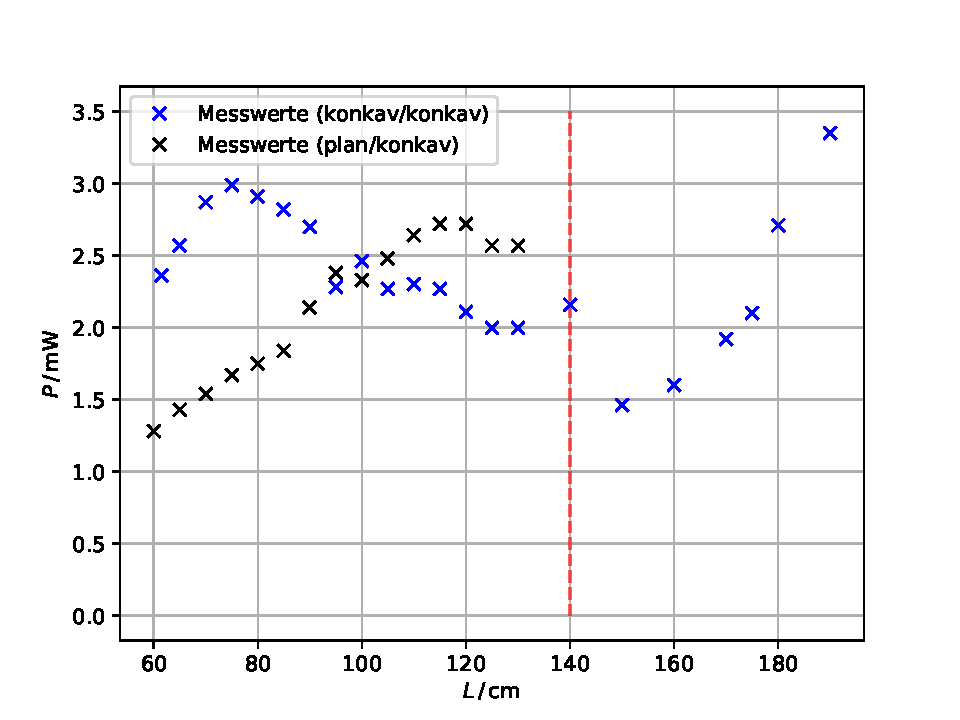
\includegraphics[width=\textwidth]{plots/leistung.pdf}
    \caption{Die gemessene Leistung $P$ in Abhängigkeit der Resonatorlänge $L$ für die beiden Speigelkonfigurationen.}
    \label{fig:leistung}
\end{figure}
\subsection{Analyse der TEM-Moden}
\subsubsection{TEM$_{00}$-Moden}
Die Leistung $P$ des Laserlichtes in Abhängigkeit von der x-Position der auf dem Schirm sichtbaren Mode lässt sich mit
einer Photodiode vermessen. Dies lässt sich mit Hilfe einer Zersteuungslinse vergrößern und erleichtert so die Messung.
Für die Grundmode $TEM_{00}$ ergibt sich nach
\begin{equation}
    I_{m0}(x)\sim H_m \left(\frac{x}{w}\right)^2\exp\left(-2\left(\frac{x}{w}\right)^2\right)
\end{equation}
mit der Hermiteschen Polynom $H_m$, die Intensitätsverteilung $I_{00}$ für die TEM$_{00}$-Mode von
\begin{equation}
    I_{00}\sim \exp\left(-2\left(\frac{x}{w}\right)^2\right)
\end{equation}

Die Leistungen in Abhängigkeit der x-Position lässt sich aus der Tabelle \ref{tab:TEM00} entnehmen.
In Abbildung \ref{fig:TEM00} sind diese Messwerte graphisch dargestellt. Darüber hinaus werden die Messwerte durch 
die Theoriefunktion interpoliert, welche die Form
\begin{equation}
    I(x)=I_0\cdot \exp\left(-2\frac{(x-x_0)^2}{w^2}\right)
\end{equation}
aufweist.
Es ergeben sich für die Parameter die Werte
\begin{align*}
    I_0&=0,031\,\text{mW}{,}\\
    x_0&=-0,32\,\text{mm}{,}\\
    w&=6,71\,\text{mm}.
\end{align*}
\begin{figure}
    \center
    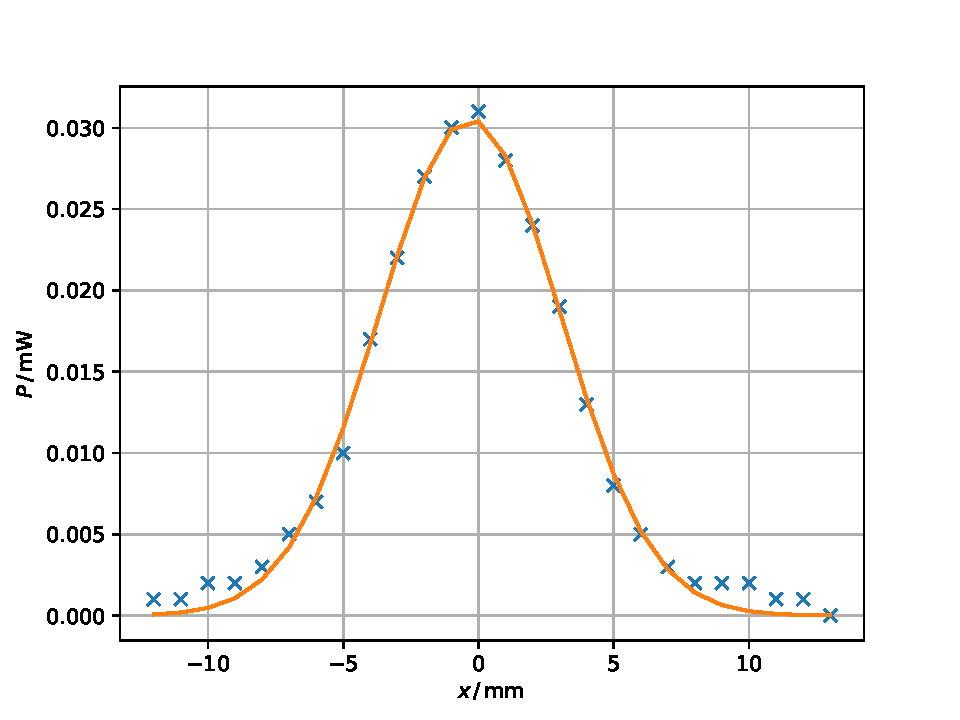
\includegraphics[width=\textwidth]{plots/TEM00.pdf}
    \caption{Die gemessene Leistung $P$ der TEM$_{00}$-Mode in Abhängigkeit der x-Position.}
    \label{fig:TEM00}
\end{figure}


\begin{table}
    \center
    \caption{Leistung $P$ der TEM$_{00}$-Mode in Abhängigkeit der x-Position.}
    \begin{tabular}{c c}
        \toprule
        $x\,/\,$mm & $P\,/\,$mW\\
        \midrule
        13&      0\\
        12&      0.001\\
        11&      0.001\\
        10&      0.002\\
        9 &      0.002\\
        8 &      0.002\\
        7 &      0.003\\
        6 &      0.005\\
        5 &      0.008\\
        4 &      0.013\\
        3 &      0.019\\
        2 &      0.024\\
        1 &      0.028\\
        0 &      0.031\\
        -1&      0.030\\
        -2&      0.027\\
        -3&      0.022\\
        -4&      0.017\\
        -5&      0.010\\
        -6&      0.007\\
        -7&      0.005\\
        -8&      0.003\\
        -9&      0.002\\
        -10&     0.002\\
        -11&     0.001\\
        -12&     0.001\\
        \bottomrule
    \end{tabular}
    \label{tab:TEM00}
\end{table}

\subsubsection{TEM$_{10}$-Moden}
Für die TEM$_{10}$-Mode folgt demnach ein $m=1$, daher ergibt sich die theoretische Intensitätsverteilung
zu 
\begin{equation}
    I(x)=I_0\cdot 4\left(\frac{(x-x_0)^2}{w^2}\right)\cdot\exp\left(-2\frac{(x-x_0)^2}{w^2}\right).
\end{equation}
Die Interpolation liefert die Werte
\begin{align*}
    I_0&=3,33\,\text{mW}{,}\\
    x_0&=0,60\,\text{mm}{,}\\
    w&=7,76\,\text{mm}.
\end{align*}
Die Leistungen $P$ zu den zugehörigen x-Positione liefern die Abbildung \ref{fig:TEM10}.
\begin{figure}
    \center
    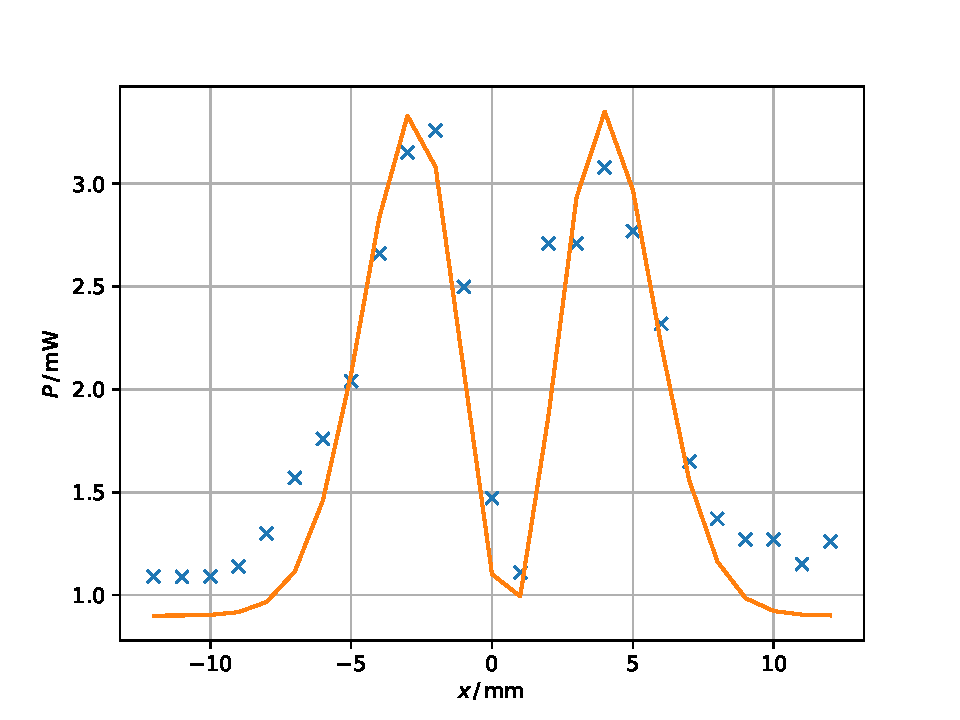
\includegraphics[width=\textwidth]{plots/TEM10.pdf}
    \caption{Die gemessene Leistung $P$ der TEM$_{10}$-Mode in Abhängigkeit der x-Position.}
    \label{fig:TEM10}
\end{figure}

\begin{table}[H]
    \center
    \caption{Leistung $P$ der TEM$_{10}$-Mode in Abhängigkeit der x-Position.}
    \begin{tabular}{c c}
        \toprule
        $x\,/\,$mm & $P\,/\,$mW\\
        \midrule
        12&      1.26\\
        11&      1.15\\
        10&      1.27\\
        9 &      1.27\\
        8 &      1.37\\
        7 &      1.65\\
        6 &      2.32\\
        5 &      2.77\\
        4 &      3.08\\
        3 &      2.71\\
        2 &      2.71\\
        1 &      1.11\\
        0 &      1.47\\
        -1&      2.499\\
        -2&      3.26\\
        -3&      3.15\\
        -4&      2.66\\
        -5&      2.04\\
        -6&      1.76\\
        -7&      1.57\\
        -8&      1.3\\
        -9&      1.14\\
        -10&     1.09\\
        -11&     1.09\\
        -12&     1.09\\
        \bottomrule
    \end{tabular}
    \label{tab:TEM10}
\end{table}

\subsection{Analyse der Polarisation}
Die gemessene Leistung $P$ in Abhängigkeit der Winkelstellung $\theta$ des Linearpolarisators ist in Tabelle \ref{tab:pol} zu finden.
Die Abhängigkeit der Intensität zum Winkel $\theta$ ergibt sich nach
\begin{equation}
    I=I_0\cos^2(\theta+\theta_0).
\end{equation}
Aus der Interpolation ergeben sich folgende Werte für die Parameter
\begin{align*}
    I_0&=1,84\,\text{mW}{,}\\
    \theta_0&=1,387\,\text{rad}{,}=79,5°.
\end{align*}
In Abbildung \ref{fig:pol} sind die Messdaten aus Tabelle \ref{tab:pol} sowie die Interpolation grafisch dargestellt.
\begin{figure}
    \center
    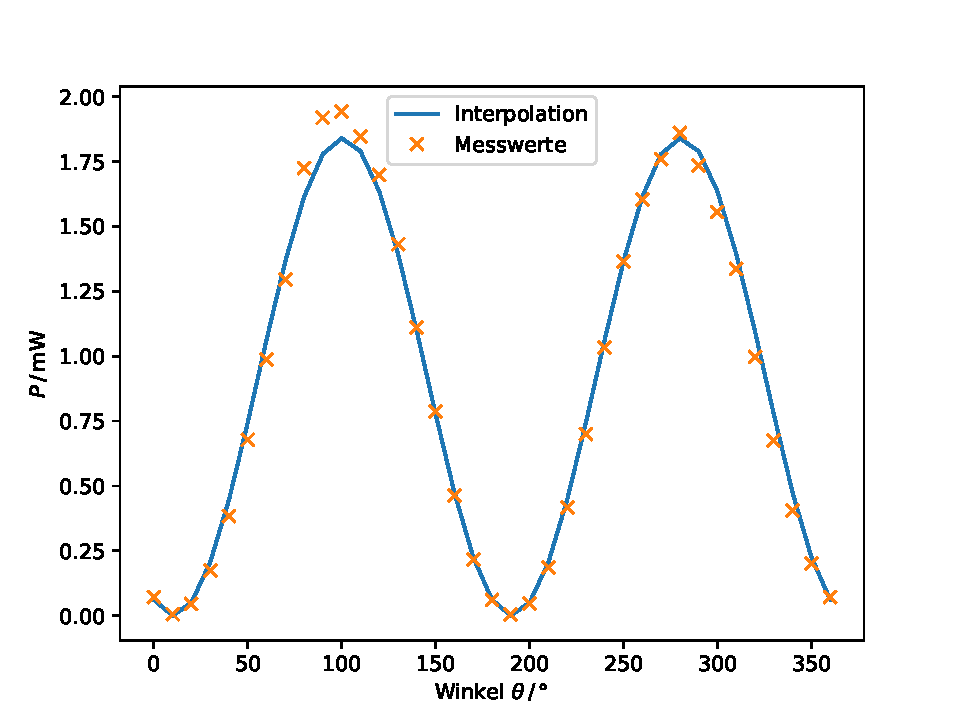
\includegraphics[width=\textwidth]{plots/pol.pdf}
    \caption{Die Leistung $P$ in Abhängigkeit des Polarisationswinkels $\theta$.}
    \label{fig:pol}
\end{figure}
\begin{table}[H]
    \center
    \caption{Die Leistung $P$ in Abhängigkeit des Polarisationswinkels $\theta$.}
    \begin{tabular}{c c}
        \toprule
        Winkel $\theta\,/\,$° & $P\,/\,$mW\\
        \midrule
        0&       0.071\\
        10&      0.006\\
        20&      0.045\\
        30&      0.174\\
        40&      0.384\\
        50&      0.678\\
        60&      0.988\\
        70&      1.295\\
        80&      1.725\\
        90&      1.920\\
        100&     1.943\\
        110&     1.848\\
        120&     1.699\\
        130&     1.431\\
        140&     1.111\\
        150&     0.787\\
        160&     0.462\\
        170&     0.217\\
        180&     0.062\\
        190&     0.005\\
        200&     0.047\\
        210&     0.186\\
        220&     0.417\\
        230&     0.7  \\
        240&     1.033\\
        250&     1.364\\
        260&     1.604\\
        270&     1.760\\
        280&     1.861\\
        290&    1.735\\
        300&     1.556\\
        310&     1.337\\
        320&     0.998\\
        330&     0.675\\
        340&     0.405\\
        350&     0.2\\
        360&     0.071\\        
        \bottomrule
    \end{tabular}
    \label{tab:pol}
\end{table}

\subsection{Analyse der Wellenlänge}
Mit Hilfe der Beugung an einem Gitter mit der Gitterkonstante $d$ können die Abstände $A_n$
der n-ten Interferenzmaxima zum Hauptmaximum $n=0$ vermessen werden. Dabei ist das Beugungsgitter
in einem Abstand $L$ zum Schirm positioniert.\\

Aus der Bedingung für eine konstruktive Interferenz nach
\begin{equation}
    \Delta g = n \cdot \lambda
\end{equation}
mit einem Gangunterschied von
\begin{equation}
    \Delta g = d \cdot \sin(\beta_n)
\end{equation}
und dem Beugungswinkel
\begin{equation}
    \beta_n=\arctan(A_n/L)
\end{equation}
ergibt sich für das n-te Maximum die Wellenlaänge $\lambda$ aus
\begin{equation}
    \lambda=\frac{d\cdot \sin(\arctan(A_n/L))}{n}=\frac{d\cdot A_n}{n\sqrt{A_n^2+L^2}}
\end{equation}
welche gemäß der gaußschen Fehlerfortpflanzung mit der Unsicherheit $\sigma(\lambda)$ behaftet ist.
Für die Fehler für die Abmessung zwischen Gitter und Schirm, seien im folgenden
\begin{equation*}
    \sigma(A_n)=\sigma(L)=5\,\text{mm}
\end{equation*}
angenommen.

\begin{table}
    \centering
    \caption{Die Berechneten Wellenlängen $\lambda$ zu den jeweiligen Vermessenden $n$-ten Beugungsmaxima der jeweiligen Gittern mit 
    den Gitterkonstanten $d$ aus dem Abstand $A_n$ zum Hauptmaxima bei einer Entfernung $L$ zum Schirm.}
    \begin{tabular}{c c c c c}
        \toprule
        Gitterkonstante $d\,/\,$mm & Ordnung $n$ & Abstand $A_n\,/\,$mm & Abstand $L\,/\,$mm & Wellenlänge $\lambda\,/\,$nm\\
        \midrule
        1/1200  &   1   &   371   &   312,5   &   637,35\\
        1/600   &   1   &   130   &   312,5   &   642,25\\
        1/600   &   2   &   379   &   312,5   &   642,95\\
        1/100   &   1   &   20      &   312,5   &   638.69\\
        1/80    &   1   &   17,5    &   312,5   &   698,90\\
        1/80    &   2   &   50      &   312,5   &   658,29\\
        1/80    &   3   &   101     &   312,5   &   643,57\\   
        \bottomrule
    \end{tabular}
    \label{tab:wellen}
\end{table}
Daraus folgt ein Mittelwert für die Wellenlänge von $\bar{\lambda}=651,71\,\text{nm}$.
